\documentclass[12pt,a4paper]{report}
\usepackage[spanish,es-tabla]{babel}
\usepackage[utf8]{inputenc}
\usepackage[T1]{fontenc}
\usepackage{geometry}
\usepackage{graphicx}
\usepackage{caption}
\usepackage{subcaption}
\usepackage{amsmath, amssymb, amsthm}
\usepackage{siunitx}
\usepackage{hyperref}
\usepackage{xcolor}
\usepackage{listings}
\usepackage{booktabs}
\usepackage{enumitem}
\usepackage{float}
\geometry{margin=1in}
\hypersetup{colorlinks=true,linkcolor=blue,urlcolor=blue,citecolor=blue}

\definecolor{codebg}{RGB}{245,245,245}
\lstdefinestyle{mypython}{
  language=Python,
  basicstyle=\ttfamily\small,
  backgroundcolor=\color{codebg},
  frame=single,
  showstringspaces=false,
  keywordstyle=\color{blue!60!black},
  commentstyle=\color{green!40!black},
  stringstyle=\color{red!60!black},
  numbers=left,
  numberstyle=\tiny, 
  stepnumber=1,
  numbersep=8pt,
  tabsize=2,
  breaklines=true,
  keepspaces=true
}

\theoremstyle{definition}
\newtheorem{definition}{Definición}
\newtheorem{remark}{Observación}

\begin{document}

\begin{titlepage}
  \centering
  {\Large Informe Académico (desde cero)}\par\vspace{0.75cm}
  {\LARGE Método de Newton--Raphson para sistemas de ecuaciones no lineales}\par
  \vspace{0.75cm}
  {\large Basado en el repositorio y figuras de `Introducción al sistema.pdf`}\par
  \vspace{1.25cm}
  {\large Fecha: \today}\par
\end{titlepage}

\tableofcontents
\clearpage

\chapter{Resumen}
Se presenta una derivación y aplicación integral del método de Newton--Raphson (NR) para resolver un sistema no lineal discreto de tamaño \(N=134\) variables, derivado de una malla \(5\times 50\) con condiciones de frontera y una viga interna. Se establecen el residual \(F(V)\), el jacobiano \(J\), el algoritmo NR, análisis de convergencia local, buenas prácticas de robustez y un esquema de implementación en Python con \texttt{numpy}/\texttt{scipy.sparse}. Se incluyen figuras tomadas de `Introducción al sistema.pdf`.

\chapter{Modelo matemático}
\section{Malla, variables y restricciones}
Sea una malla rectangular de \(5\) filas por \(50\) columnas. Se definen velocidades \(V_{i,j}\) por nodo. Las condiciones de frontera fijan valores en suelo, superficie, entrada y salida; adicionalmente, una viga fija 10 nodos en \(j=1\), \(i\in[20,29]\). Las incógnitas corresponden a los nodos restantes, total \(N=134\).

\begin{figure}[H]
  \centering
  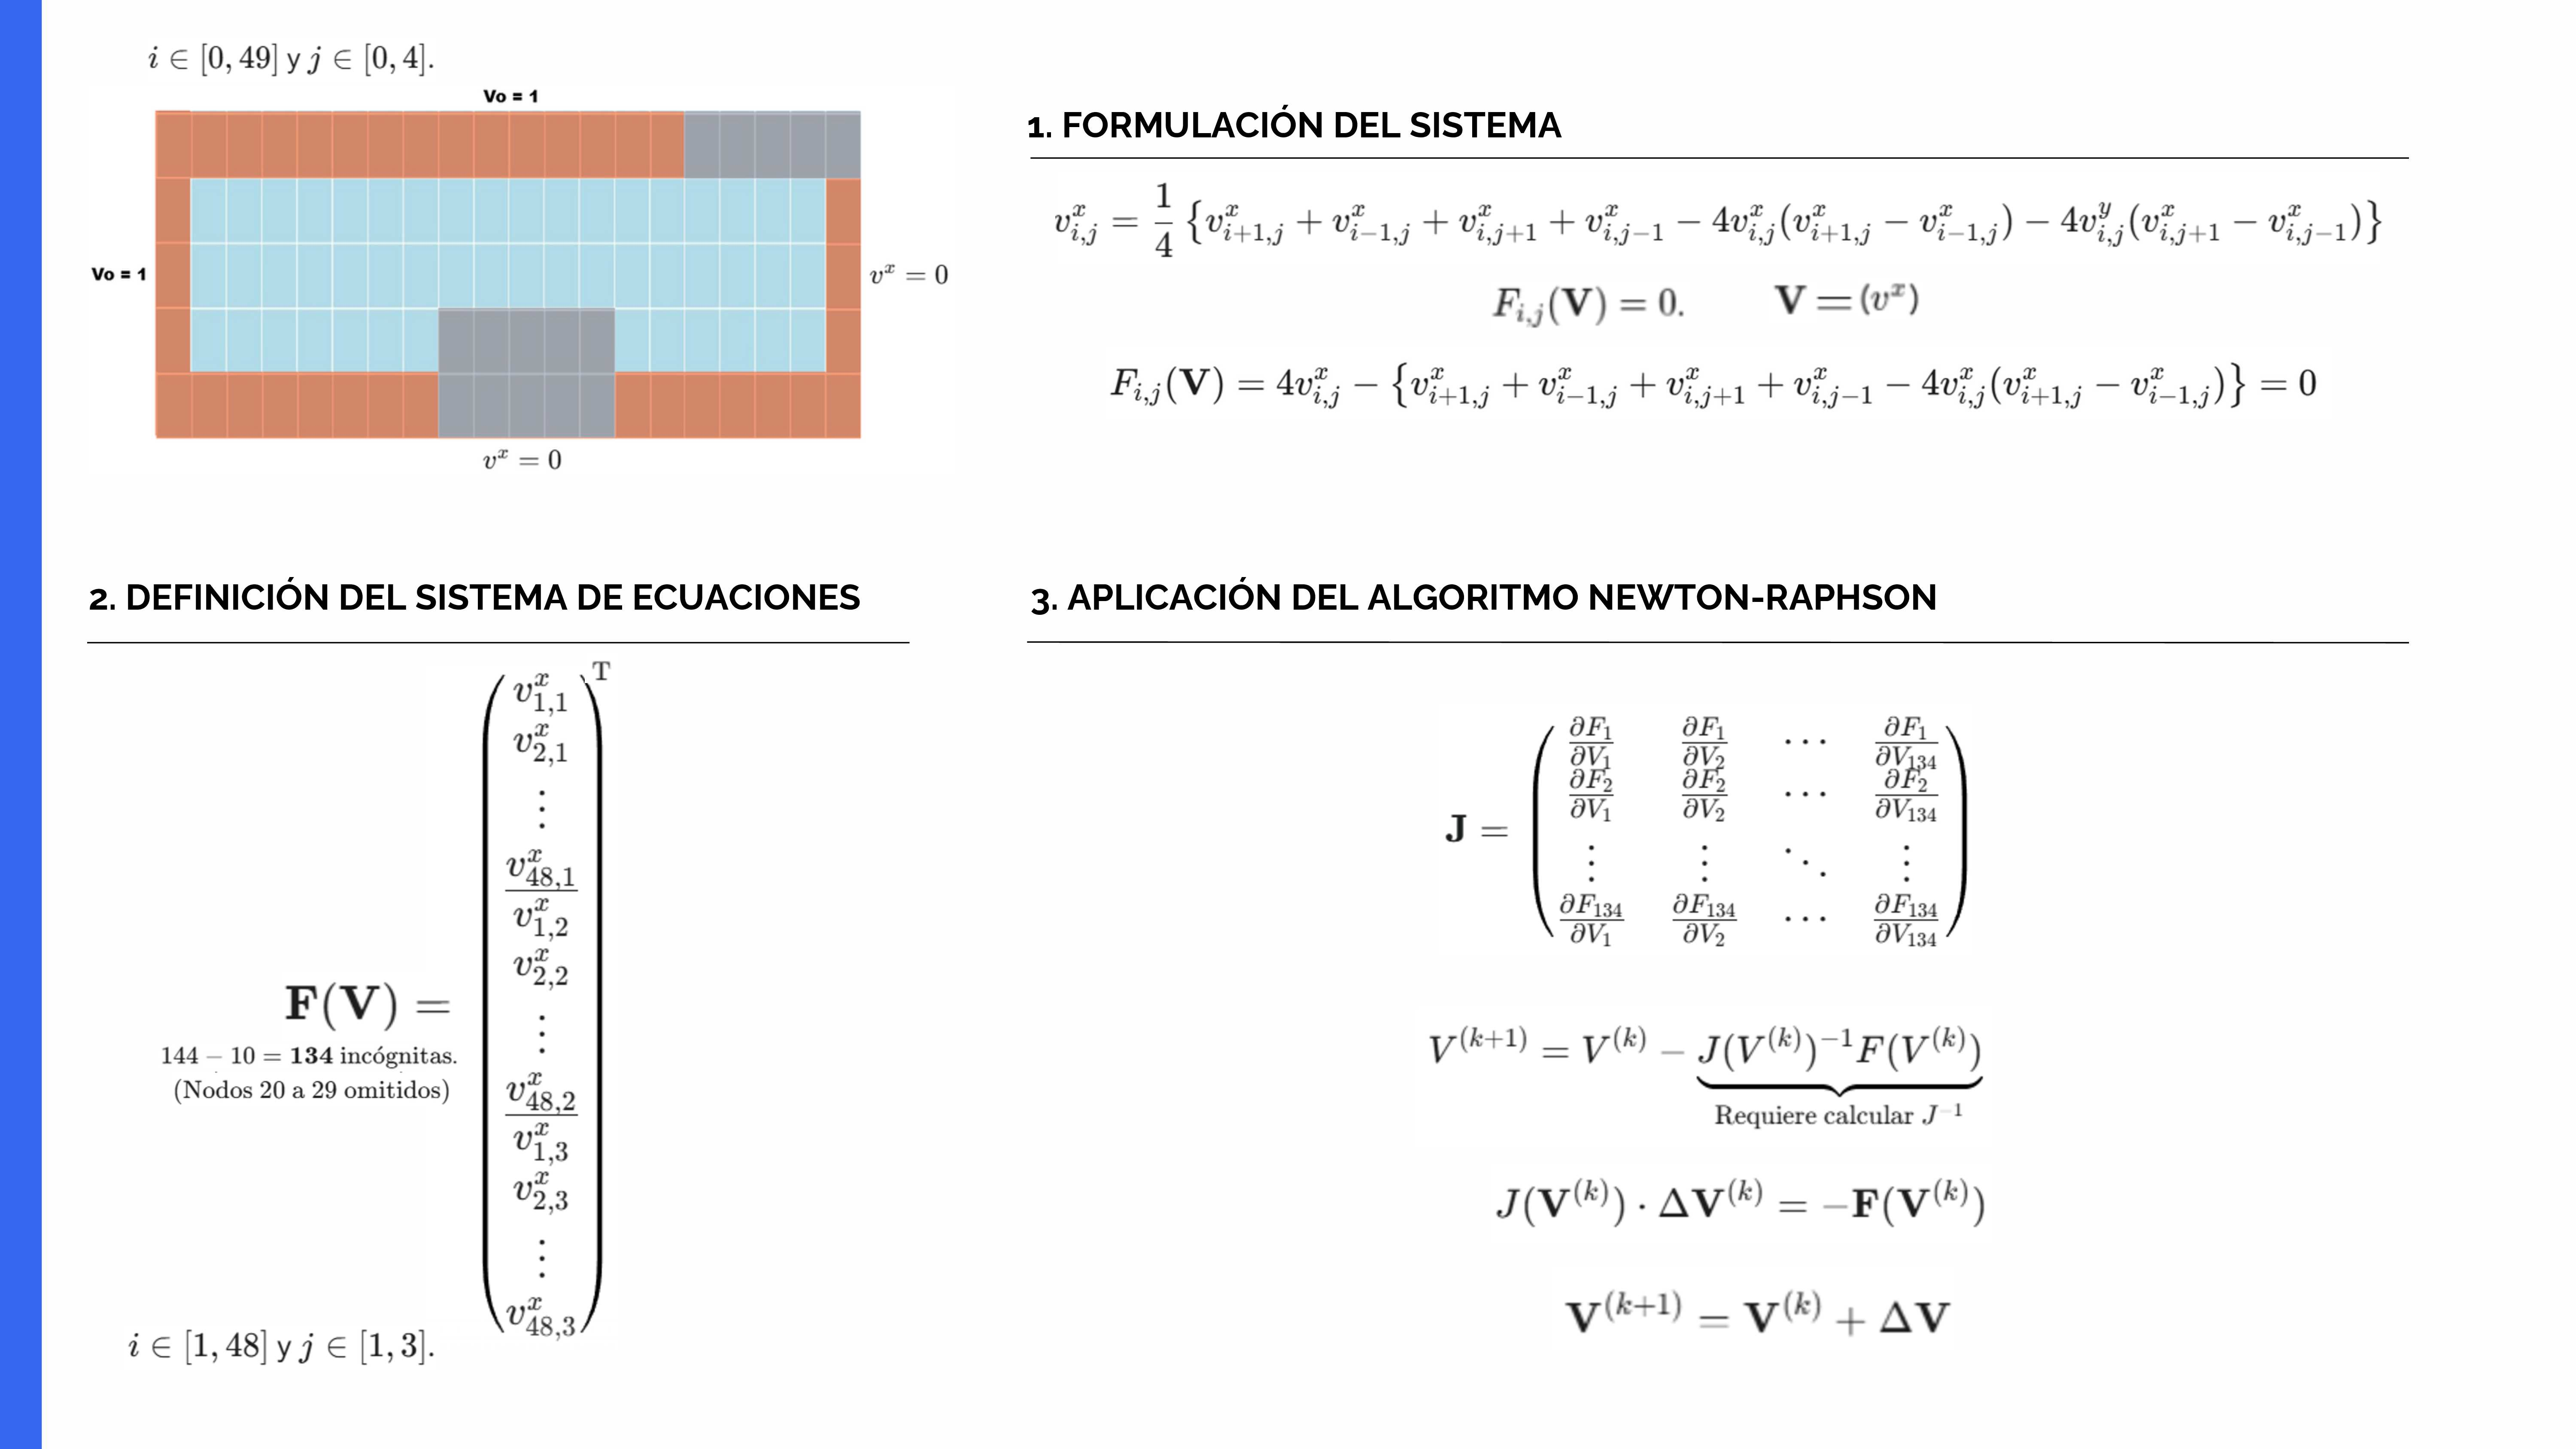
\includegraphics[width=0.95\textwidth]{intro_img-001.png}
  \caption{Conteo de incógnitas y esquema del residual (de `Introducción al sistema.pdf`).}
\end{figure}

\section{Residual no lineal}
Para cada nodo interior \((i,j)\), el equilibrio se expresa como \(F_{i,j}(V)=0\). Un modelo representativo (difusión + convección) es:
\begin{equation}
\label{eq:res}
\small
F_{i,j}(V) = 4\,V_{i,j} - (V_{i+1,j}+V_{i-1,j}+V_{i,j+1}+V_{i,j-1}) 
              + c\,V_{i,j}\,V_{i-1,j} - c\,V_{i,j}\,V_{i+1,j},
\end{equation}
con \(c>0\) el parámetro convectivo. Apilando las ecuaciones sobre incógnitas se obtiene \(F: \mathbb{R}^{N}\to\mathbb{R}^{N}\).

\section{Jacobiano}
El jacobiano \(J=\partial F/\partial V\) se ensambla por derivación de \eqref{eq:res} respecto de las cinco variables locales: nodo central y sus cuatro vecinos. Esto produce una matriz esparsa de tamaño \(N\times N\) con a lo sumo cinco entradas no nulas por fila (menor cerca de fronteras/viga).

\begin{figure}[H]
  \centering
  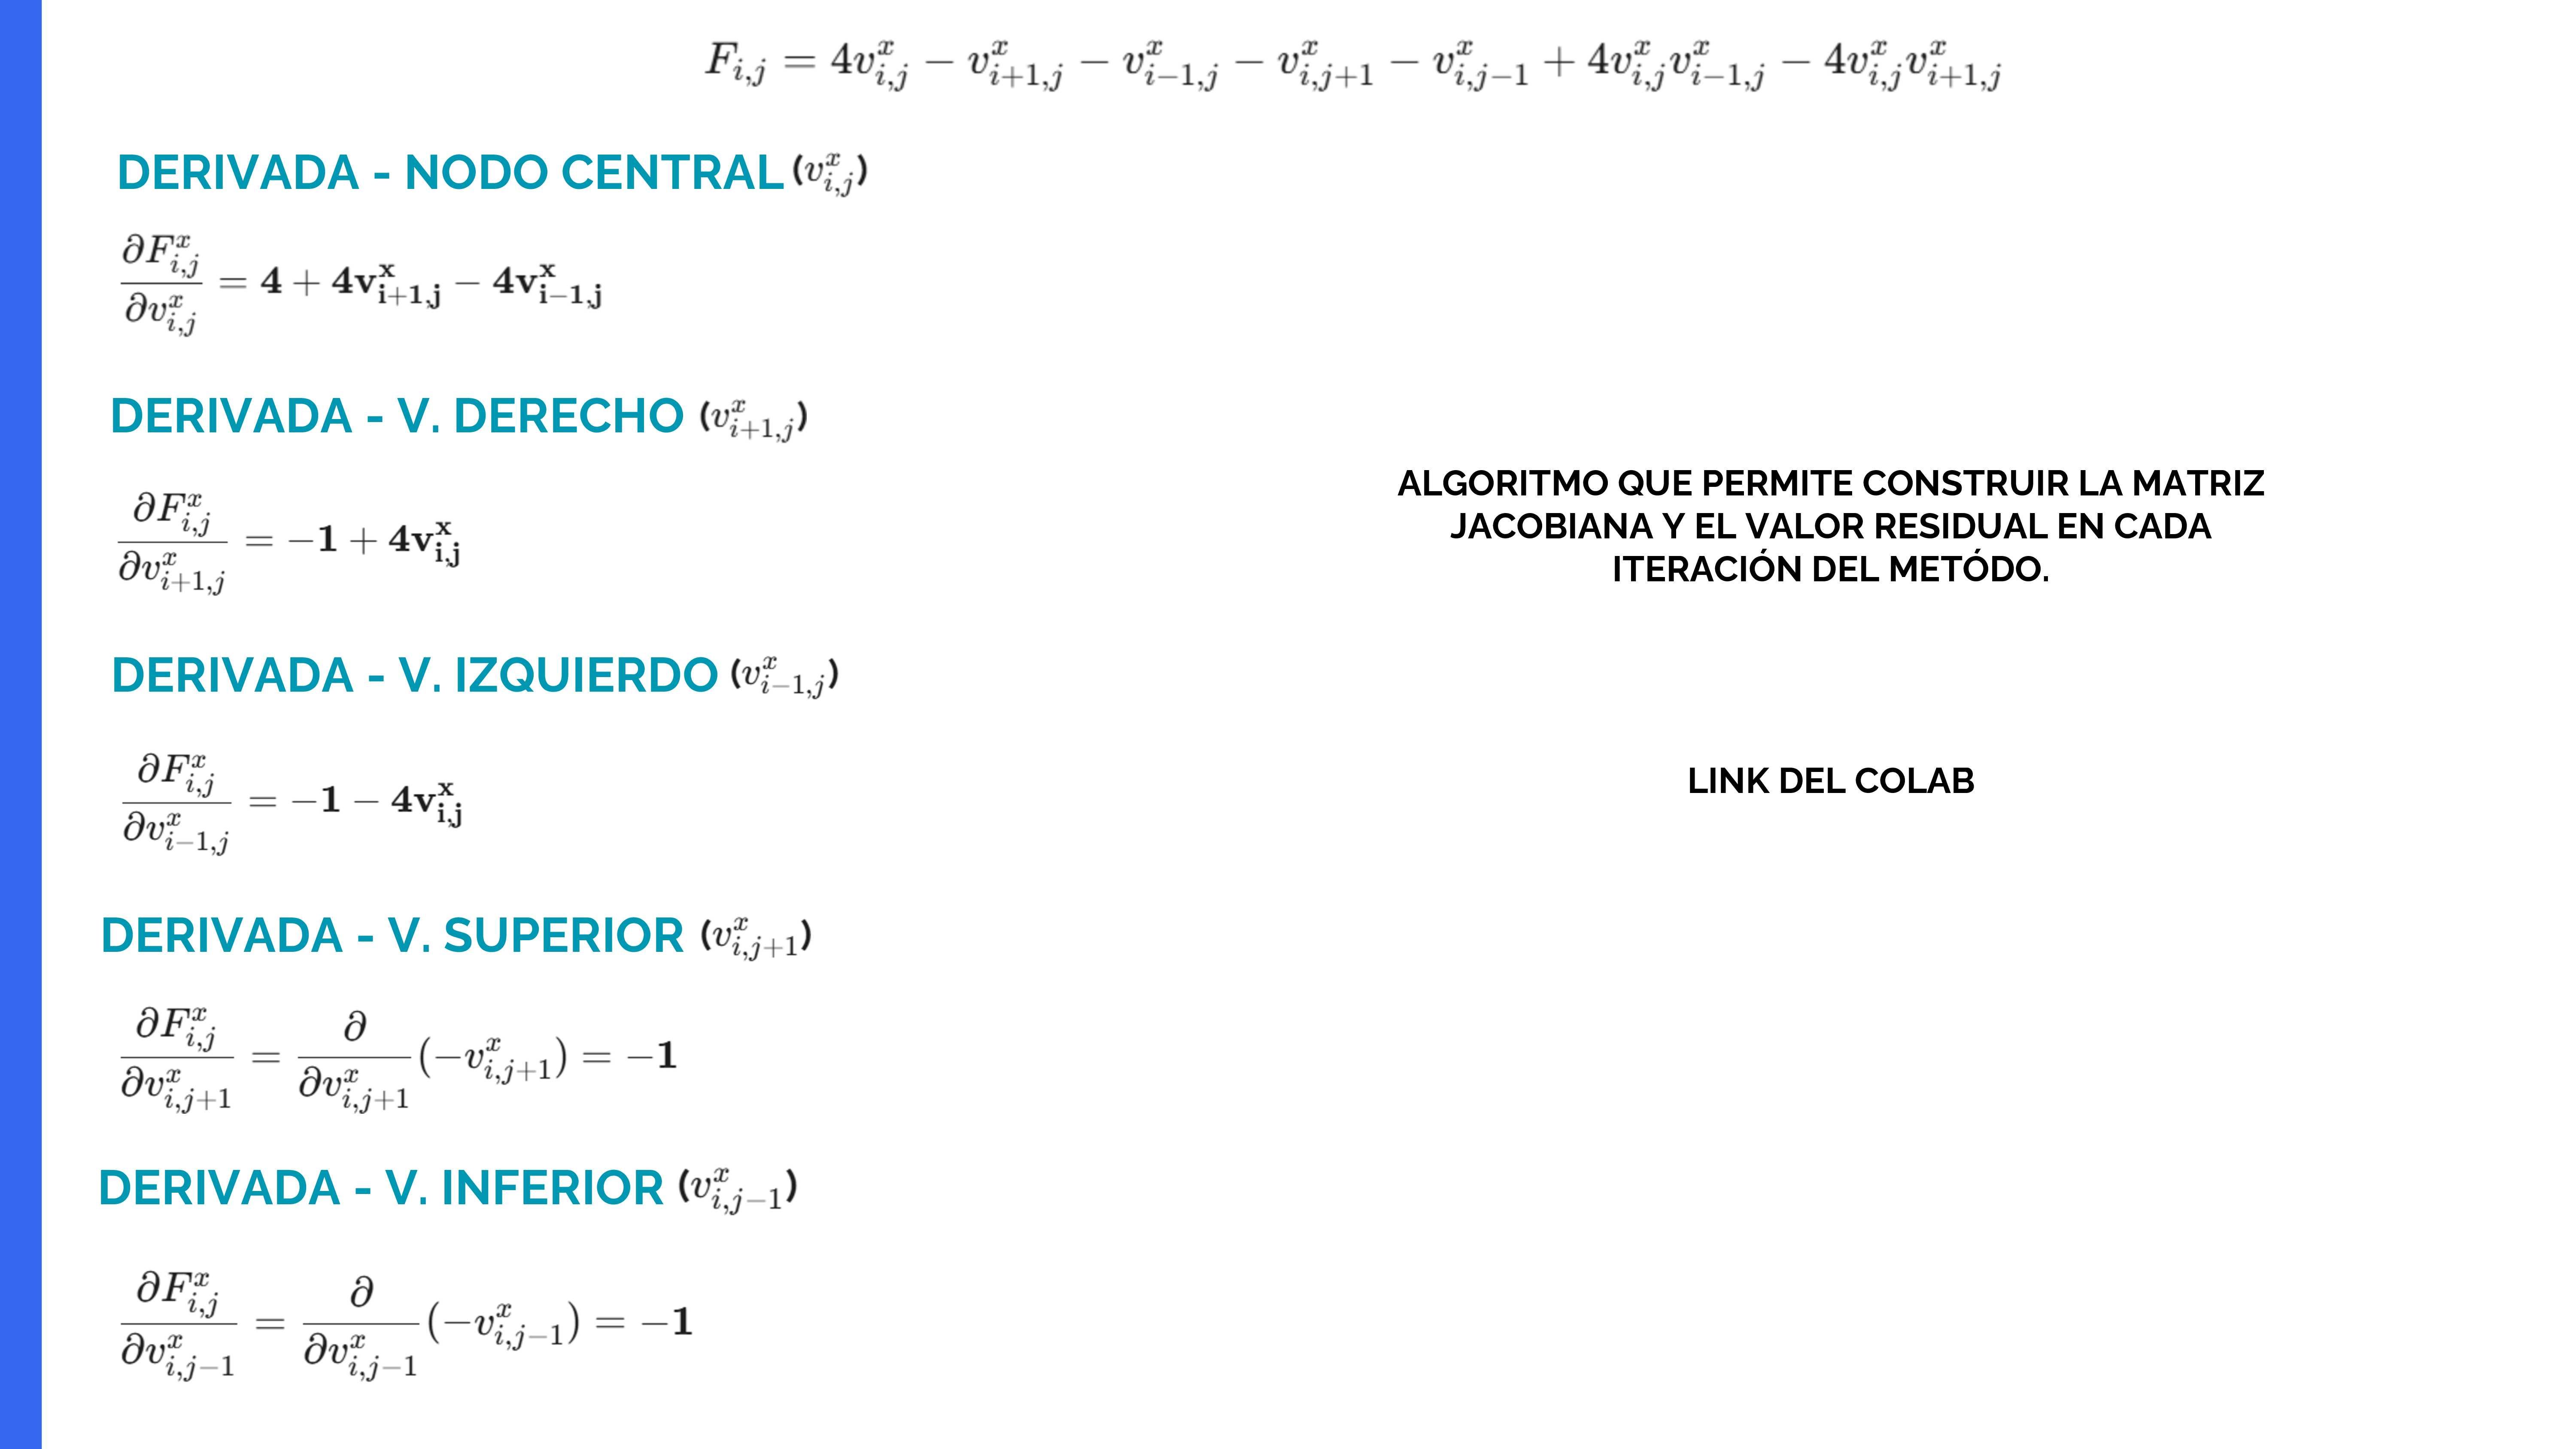
\includegraphics[width=0.95\textwidth]{intro_img-002.png}
  \caption{Derivadas parciales para el jacobiano (de `Introducción al sistema.pdf`).}
\end{figure}

\chapter{Método de Newton--Raphson}
\section{Esquema}
Dado \(V^{(k)}\), el paso NR resuelve
\begin{equation*}
J(V^{(k)})\,\Delta V^{(k)} = -F(V^{(k)}),\qquad V^{(k+1)} = V^{(k)} + \Delta V^{(k)}.
\end{equation*}
\section{Algoritmo}
\begin{enumerate}[label=\arabic*.]
  \item Elegir \(V^{(0)}\) (p.ej., constante en nodos internos).
  \item Repetir hasta convergencia:
  \begin{enumerate}[label=\alph*)]
    \item Ensamblar \(F\) y \(J\).
    \item Resolver \(J\,\Delta V= -F\) (solver esparso).
    \item Actualizar \(V\leftarrow V+\Delta V\).
    \item Comprobar \(\|F\|\) y/o \(\|\Delta V\|\) contra tolerancias.
  \end{enumerate}
\end{enumerate}

\section{Convergencia}
Si \(V^{(0)}\) es cercano a la solución y \(J\) es no singular en la raíz, NR exhibe convergencia local cuadrática. En presencia de fuertes no linealidades convectivas, puede requerirse \emph{damping} o búsqueda lineal.

\chapter{Implementación propuesta}
\section{Estructura de datos y mapeo}
\begin{lstlisting}[style=mypython]
import numpy as np
from scipy.sparse import lil_matrix, linalg

J_MAX, I_MAX = 3, 48
N = 134
V0, C = 1.0, 4.0

# Fronteras y viga
# (Devuelve None si es incógnita; valor numérico si es nodo fijo)

def get_bc(i, j):
    if (j == 1 and 20 <= i <= 29):
        return 0.0
    if j == 0:
        return 0.0
    if j == 4:
        return V0
    if i == 0:
        return V0
    if i == 49:
        return 0.0
    return None

# Mapeo (i,j) -> índice plano en [0..N-1], omitiendo fijos y viga

def to_index(i, j):
    if get_bc(i, j) is not None:
        return -1
    base_j = 48 * (j - 1)
    idx_i = i - 1
    shift_viga = 0
    if j == 1:
        if i >= 30:
            shift_viga = 10
        elif 20 <= i <= 29:
            return -1
    if j == 2:
        base_j = 38
    elif j == 3:
        base_j = 86
    idx = base_j + idx_i - shift_viga
    return idx if 0 <= idx < N else -1

# Acceso a V con fronteras

def V_at(i, j, V):
    bc = get_bc(i, j)
    if bc is not None:
        return bc
    p = to_index(i, j)
    return V[p] if p != -1 else 0.0
\end{lstlisting}

\section{Ensamblaje de \(F\) y \(J\)}
\begin{lstlisting}[style=mypython]

def assemble_FJ(V):
    J = lil_matrix((N, N), dtype=np.float64)
    F = np.zeros(N)

    for j in range(1, J_MAX + 1):
        for i in range(1, I_MAX + 1):
            m = to_index(i, j)
            if m == -1:
                continue
            Vij   = V[m]
            Vip1j = V_at(i + 1, j, V)
            Vim1j = V_at(i - 1, j, V)
            Vijp1 = V_at(i, j + 1, V)
            Vijm1 = V_at(i, j - 1, V)

            # Residual (difusión + convección)
            F[m] = (4.0 * Vij
                    - (Vip1j + Vim1j + Vijp1 + Vijm1)
                    + (C * Vij * Vim1j)
                    - (C * Vij * Vip1j))

            # Parciales (jacobiano)
            J[m, m] = 4.0 + (C * Vim1j) - (C * Vip1j)
            r = to_index(i + 1, j)
            if r != -1:
                J[m, r] = -1.0 - (C * Vij)
            l = to_index(i - 1, j)
            if l != -1:
                J[m, l] = -1.0 + (C * Vij)
            u = to_index(i, j + 1)
            if u != -1:
                J[m, u] = -1.0
            d = to_index(i, j - 1)
            if d != -1:
                J[m, d] = -1.0

    return J.tocsr(), F
\end{lstlisting}

\section{Iteraciones NR}
\begin{lstlisting}[style=mypython]

def newton_raphson():
    V = np.ones(N) * V0
    TOL = 1e-6
    MAXIT = 100
    for k in range(MAXIT):
        J, F = assemble_FJ(V)
        if np.linalg.norm(F) < TOL:
            break
        dV = linalg.spsolve(J, -F)
        V += dV
        if np.linalg.norm(dV) < TOL:
            break
    return V
\end{lstlisting}

\chapter{Buenas prácticas y validación}
\begin{itemize}
  \item Validación de \(J\) con diferencias finitas puntuales.
  \item Registro de \(\|F\|\) y \(\|\Delta V\|\) por iteración.
  \item Damping o búsqueda lineal ante oscilaciones.
  \item Visualización del campo \(V\) (\texttt{matplotlib}) y comparación cualitativa.
\end{itemize}

\chapter{Conclusiones}
Se construyó un informe académico formal, desde cero, que detalla residual, jacobiano, algoritmo NR y una propuesta de implementación esparsa. Las figuras de `Introducción al sistema.pdf` contextualizan el conteo de incógnitas y la estructura del jacobiano.

\end{document}
